\section{Stage 1: Winch Activation}

Since recovering lost cable length can be difficult and timely to recover, there should be a strong indication that the traction control architecture alone can not maintain tractor mobility before using the winch. At the same time, waiting too long to activate the winch could result in the tractor becoming stuck and excavating itself into the terrain. To strike a balance between both concerns, the bounds on the terrain parameter space and their resulting slip-force curves are used as a guide. In section \ref{ch:TCM},
Fig. \ref{s:TCMA} shows a histogram of the peak slip points $i_{pk}$ for all terrain hypothesis models. The largest value shown is $i_{pk} \simeq 41\%$. Therefore, once the DTKF estimates a value of $\hat{i} \geq 45\%$, this is an indication that using the traction control mode alone can not maintain tractor mobility and the winch is activated to let out payload and reduce drawbar load. 

The starting position of the 4 way, 2 position valve in the winch hydraulics is shown in Fig. \ref{fig:WINCH_HYDRAULICS_DIAGRAM_VP2} before winch activation. This position is maintained once the control mode has been activated however the $P_{set}$ value transitions from $P_{set} = 2700\hspace{1mm}psi$ to $P_{set} = 0\hspace{1mm}psi$ in eq. \ref{eq:VP2_eq4} for the braking valve B2. This allows more hydraulic fluid to flow out of the $P_O$ node to reduce fluid pressure and subsequently the braking torque $\tau_W$.
\begin{figure}[htb]
    \centering
    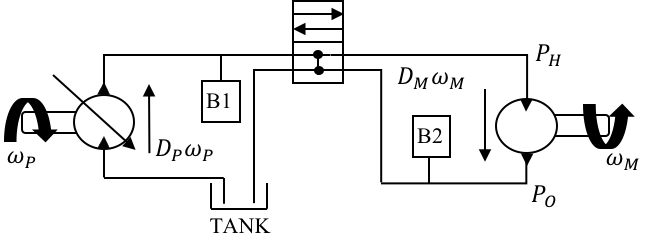
\includegraphics[width = 4in, keepaspectratio]{WINCH_HYDRAULICS_DIAGRAM_VP2}
    \caption{Starting position of the 4 way, 2 position valve when the winch is activated in the winch control mode. The braking valve $p_{set} = 2700\hspace{1mm}psi$ before the mode is activated and is lowered to $p_{set} = 0\hspace{1mm}psi$ once the mobility issues have been detected and the control mode is activated. This reduces the braking torque of the winch so that cable can be let out to reduce drawbar load.}
    \label{fig:WINCH_HYDRAULICS_DIAGRAM_VP2}
\end{figure}


